\section{Camera Intrinsic Calibration}
\label{section:camera-intrinsic-calibration}

The intrinsic calibration determines the intrinsic parameters of the camera, such as the focal lenght ($f = (f_x, f_y)$), the optical center ($c = (c_x, c_y)$) and the distortion coefficients to model the lens distortion. This parameters are required to create the distortion matrix, as well as the undistortion function, which is essencial for the point projection (as described in \cref{section:color-registration}).

The calibration procedure used in this work is a standard procedure for cameras with low distortion and is known as the chessboard camera calibration. This method calibrates a monocular camera with fixed focus using a sequence of images taken from a chessboard with known dimensions. In order to improve the calibration results, the chessboard should rotate and move, in order to occupy the entire image size.

After all the images are obtained, the corners of the chessboard are extracted and the re-projection error is minimized to obtain the the intrinsic parameters. The results of this calibration are more accurate if the corners of the chessboard are well defined in the image, so the chessboard should have an appropriate size. Also, the chessboard poses should be enough and should be well distributed spatially.

In the end, the accuracy of the calibration should be measured for new images, with the re-projection error. This value should be as low as possible and, as a rule of thumb, a value less than \num{0.01} is acceptable.

In ROS, this calibration is easily obtained with the \emph{cameracalibrator.py}, which includes a graphical interface, and provides feedback about the corner detection and the state of the calibration. The interface is shown on \cref{figure:camera-calibrator}. In this system, this data is first saved into a ROS \emph{camera\_info} file. Then, this file is also saved in each capture in the parameters file.

\begin{figure}
    
    \centering
    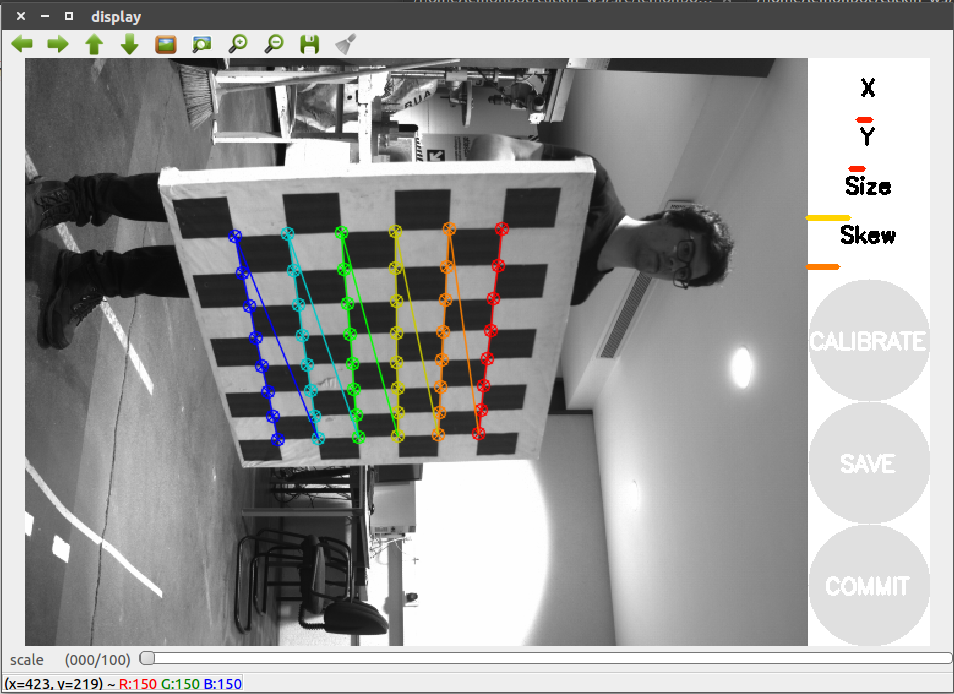
\includegraphics[width=10cm]{camera-intrinsic-calibration}

    \caption{Interface for the \emph{cameracalibrator} node}
    \label{figure:camera-calibrator}

\end{figure}